\documentclass[11pt,addpoints,answers]{exam}
%-----------------------------------------------------------------------------
% PACKAGES AND OTHER DOCUMENT CONFIGURATIONS
%-----------------------------------------------------------------------------

\usepackage[margin=1in]{geometry}
\usepackage{amsmath, amsfonts}
\usepackage{enumerate}
\usepackage{graphicx}
\usepackage{titling}
\usepackage{url}
\usepackage{xfrac}
\usepackage{natbib}
\usepackage{amssymb}
\usepackage{amsthm}
\usepackage{paralist}
\usepackage{epstopdf}
\usepackage{tabularx}
\usepackage{longtable}
\usepackage{multirow}
\usepackage{multicol}
\usepackage[colorlinks=true,urlcolor=blue]{hyperref}
\usepackage{algorithm}
\usepackage{algorithmicx}
\usepackage[noend]{algpseudocode}
\usepackage{float}
\usepackage{enumerate}
\usepackage{array}
\usepackage{environ}
\usepackage{times}
\usepackage{textcomp}
\usepackage{caption}
\usepackage{parskip} % For NIPS style paragraphs.
\usepackage[compact]{titlesec} % Less whitespace around titles
\usepackage{titling}
\setlength{\droptitle}{-2cm}
\usepackage[inline]{enumitem} % For inline enumerate* and itemize*
\usepackage{datetime}
\usepackage{comment}
% \usepackage{minted}
\usepackage{lastpage}
\usepackage{color}
\usepackage[dvipsnames]{xcolor}
\usepackage[final]{listings}
\usepackage{tikz}
\usetikzlibrary{shapes,decorations}
\usepackage{framed}
\usepackage{booktabs}
\usepackage{cprotect}
\usepackage{verbatimbox}
\usepackage{multicol}
\usepackage{hyperref}
\usepackage{subcaption}
\usepackage{mathtools} % For drcases
\usepackage{cancel}
\usepackage[many]{tcolorbox}
\usepackage{soul}
\usepackage{tikz}
\usepackage{wasysym}
\usepackage{mdsymbol}
\usepackage{transparent}
\usepackage{bm}

\usetikzlibrary{shapes.geometric}
\usetikzlibrary{positioning, arrows, automata}


%%%%%%%%%%%%%%%%%%%%%%%%%%%%%%%%%%%%%%%%%%
% Custom commands                        %
%%%%%%%%%%%%%%%%%%%%%%%%%%%%%%%%%%%%%%%%%%

\newcommand{\vc}[1]{\boldsymbol{#1}}
\newcommand{\adj}[1]{\frac{d J}{d #1}}
\newcommand{\chain}[2]{\adj{#2} = \adj{#1}\frac{d #1}{d #2}}

% mathcal
\newcommand{\Ac}{\mathcal{A}}
\newcommand{\Bc}{\mathcal{B}}
\newcommand{\Cc}{\mathcal{C}}
\newcommand{\Dc}{\mathcal{D}}
\newcommand{\Ec}{\mathcal{E}}
\newcommand{\Fc}{\mathcal{F}}
\newcommand{\Gc}{\mathcal{G}}
\newcommand{\Hc}{\mathcal{H}}
\newcommand{\Ic}{\mathcal{I}}
\newcommand{\Jc}{\mathcal{J}}
\newcommand{\Kc}{\mathcal{K}}
\newcommand{\Lc}{\mathcal{L}}
\newcommand{\Mc}{\mathcal{M}}
\newcommand{\Nc}{\mathcal{N}}
\newcommand{\Oc}{\mathcal{O}}
\newcommand{\Pc}{\mathcal{P}}
\newcommand{\Qc}{\mathcal{Q}}
\newcommand{\Rc}{\mathcal{R}}
\newcommand{\Sc}{\mathcal{S}}
\newcommand{\Tc}{\mathcal{T}}
\newcommand{\Uc}{\mathcal{U}}
\newcommand{\Vc}{\mathcal{V}}
\newcommand{\Wc}{\mathcal{W}}
\newcommand{\Xc}{\mathcal{X}}
\newcommand{\Yc}{\mathcal{Y}}
\newcommand{\Zc}{\mathcal{Z}}

% mathbb
\newcommand{\Ab}{\mathbb{A}}
\newcommand{\Bb}{\mathbb{B}}
\newcommand{\Cb}{\mathbb{C}}
\newcommand{\Db}{\mathbb{D}}
\newcommand{\Eb}{\mathbb{E}}
\newcommand{\Fb}{\mathbb{F}}
\newcommand{\Gb}{\mathbb{G}}
\newcommand{\Hb}{\mathbb{H}}
\newcommand{\Ib}{\mathbb{I}}
\newcommand{\Jb}{\mathbb{J}}
\newcommand{\Kb}{\mathbb{K}}
\newcommand{\Lb}{\mathbb{L}}
\newcommand{\Mb}{\mathbb{M}}
\newcommand{\Nb}{\mathbb{N}}
\newcommand{\Ob}{\mathbb{O}}
\newcommand{\Pb}{\mathbb{P}}
\newcommand{\Qb}{\mathbb{Q}}
\newcommand{\Rb}{\mathbb{R}}
\newcommand{\Sb}{\mathbb{S}}
\newcommand{\Tb}{\mathbb{T}}
\newcommand{\Ub}{\mathbb{U}}
\newcommand{\Vb}{\mathbb{V}}
\newcommand{\Wb}{\mathbb{W}}
\newcommand{\Xb}{\mathbb{X}}
\newcommand{\Yb}{\mathbb{Y}}
\newcommand{\Zb}{\mathbb{Z}}

% mathbf lowercase
\newcommand{\av}{\mathbf{a}}
\newcommand{\bv}{\mathbf{b}}
\newcommand{\cv}{\mathbf{c}}
\newcommand{\dv}{\mathbf{d}}
\newcommand{\ev}{\mathbf{e}}
\newcommand{\fv}{\mathbf{f}}
\newcommand{\gv}{\mathbf{g}}
\newcommand{\hv}{\mathbf{h}}
\newcommand{\iv}{\mathbf{i}}
\newcommand{\jv}{\mathbf{j}}
\newcommand{\kv}{\mathbf{k}}
\newcommand{\lv}{\mathbf{l}}
\newcommand{\mv}{\mathbf{m}}
\newcommand{\nv}{\mathbf{n}}
\newcommand{\ov}{\mathbf{o}}
\newcommand{\pv}{\mathbf{p}}
\newcommand{\qv}{\mathbf{q}}
\newcommand{\rv}{\mathbf{r}}
\newcommand{\sv}{\mathbf{s}}
\newcommand{\tv}{\mathbf{t}}
\newcommand{\uv}{\mathbf{u}}
\newcommand{\vv}{\mathbf{v}}
\newcommand{\wv}{\mathbf{w}}
\newcommand{\xv}{\mathbf{x}}
\newcommand{\yv}{\mathbf{y}}
\newcommand{\zv}{\mathbf{z}}

% mathbf uppercase
\newcommand{\Av}{\mathbf{A}}
\newcommand{\Bv}{\mathbf{B}}
\newcommand{\Cv}{\mathbf{C}}
\newcommand{\Dv}{\mathbf{D}}
\newcommand{\Ev}{\mathbf{E}}
\newcommand{\Fv}{\mathbf{F}}
\newcommand{\Gv}{\mathbf{G}}
\newcommand{\Hv}{\mathbf{H}}
\newcommand{\Iv}{\mathbf{I}}
\newcommand{\Jv}{\mathbf{J}}
\newcommand{\Kv}{\mathbf{K}}
\newcommand{\Lv}{\mathbf{L}}
\newcommand{\Mv}{\mathbf{M}}
\newcommand{\Nv}{\mathbf{N}}
\newcommand{\Ov}{\mathbf{O}}
\newcommand{\Pv}{\mathbf{P}}
\newcommand{\Qv}{\mathbf{Q}}
\newcommand{\Rv}{\mathbf{R}}
\newcommand{\Sv}{\mathbf{S}}
\newcommand{\Tv}{\mathbf{T}}
\newcommand{\Uv}{\mathbf{U}}
\newcommand{\Vv}{\mathbf{V}}
\newcommand{\Wv}{\mathbf{W}}
\newcommand{\Xv}{\mathbf{X}}
\newcommand{\Yv}{\mathbf{Y}}
\newcommand{\Zv}{\mathbf{Z}}

% bold greek lowercase
\newcommand{\alphav     }{\boldsymbol \alpha     }
\newcommand{\betav      }{\boldsymbol \beta      }
\newcommand{\gammav     }{\boldsymbol \gamma     }
\newcommand{\deltav     }{\boldsymbol \delta     }
\newcommand{\epsilonv   }{\boldsymbol \epsilon   }
\newcommand{\varepsilonv}{\boldsymbol \varepsilon}
\newcommand{\zetav      }{\boldsymbol \zeta      }
\newcommand{\etav       }{\boldsymbol \eta       }
\newcommand{\thetav     }{\boldsymbol \theta     }
\newcommand{\varthetav  }{\boldsymbol \vartheta  }
\newcommand{\iotav      }{\boldsymbol \iota      }
\newcommand{\kappav     }{\boldsymbol \kappa     }
\newcommand{\varkappav  }{\boldsymbol \varkappa  }
\newcommand{\lambdav    }{\boldsymbol \lambda    }
\newcommand{\muv        }{\boldsymbol \mu        }
\newcommand{\nuv        }{\boldsymbol \nu        }
\newcommand{\xiv        }{\boldsymbol \xi        }
\newcommand{\omicronv   }{\boldsymbol \omicron   }
\newcommand{\piv        }{\boldsymbol \pi        }
\newcommand{\varpiv     }{\boldsymbol \varpi     }
\newcommand{\rhov       }{\boldsymbol \rho       }
\newcommand{\varrhov    }{\boldsymbol \varrho    }
\newcommand{\sigmav     }{\boldsymbol \sigma     }
\newcommand{\varsigmav  }{\boldsymbol \varsigma  }
\newcommand{\tauv       }{\boldsymbol \tau       }
\newcommand{\upsilonv   }{\boldsymbol \upsilon   }
\newcommand{\phiv       }{\boldsymbol \phi       }
\newcommand{\varphiv    }{\boldsymbol \varphi    }
\newcommand{\chiv       }{\boldsymbol \chi       }
\newcommand{\psiv       }{\boldsymbol \psi       }
\newcommand{\omegav     }{\boldsymbol \omega     }

% bold greek uppercase
\newcommand{\Gammav     }{\boldsymbol \Gamma     }
\newcommand{\Deltav     }{\boldsymbol \Delta     }
\newcommand{\Thetav     }{\boldsymbol \Theta     }
\newcommand{\Lambdav    }{\boldsymbol \Lambda    }
\newcommand{\Xiv        }{\boldsymbol \Xi        }
\newcommand{\Piv        }{\boldsymbol \Pi        }
\newcommand{\Sigmav     }{\boldsymbol \Sigma     }
\newcommand{\Upsilonv   }{\boldsymbol \Upsilon   }
\newcommand{\Phiv       }{\boldsymbol \Phi       }
\newcommand{\Psiv       }{\boldsymbol \Psi       }
\newcommand{\Omegav     }{\boldsymbol \Omega     }


\newtcolorbox[]{your_solution}[1][]{%
    % breakable,
    enhanced,
    nobeforeafter,
    colback=white,
    title=Your Answer,
    sidebyside align=top,
    box align=top,
    #1
}

%%%%%%%%%%%%%%%%%%%%%%%%%%%%%%%%%%%%%%%%%%%
% Better numbering                        %
%%%%%%%%%%%%%%%%%%%%%%%%%%%%%%%%%%%%%%%%%%%

% \numberwithin{equation}{section} % Number equations within sections (i.e. 1.1, 1.2, 2.1, 2.2 instead of 1, 2, 3, 4)
% \numberwithin{figure}{section} % Number figures within sections (i.e. 1.1, 1.2, 2.1, 2.2 instead of 1, 2, 3, 4)
% \numberwithin{table}{section} % Number tables within sections (i.e. 1.1, 1.2, 2.1, 2.2 instead of 1, 2, 3, 4)

%%%%%%%%%%%%%%%%%%%%%%%%%%%%%%%%%%%%%%%%%%
% Custom commands                        %
%%%%%%%%%%%%%%%%%%%%%%%%%%%%%%%%%%%%%%%%%%
\newcommand{\blackcircle}{\tikz\draw[black,fill=black] (0,0) circle (1ex);}
\renewcommand{\circle}{\tikz\draw[black] (0,0) circle (1ex);}
\newcommand{\ntset}{test}

%%%%%%%%%%%%%%%%%%%%%%%%%%%%%%%%%%%%%%%%%%%
% Code highlighting with listings         %
%%%%%%%%%%%%%%%%%%%%%%%%%%%%%%%%%%%%%%%%%%%

\definecolor{bluekeywords}{rgb}{0.13,0.13,1}
\definecolor{greencomments}{rgb}{0,0.5,0}
\definecolor{redstrings}{rgb}{0.9,0,0}
\definecolor{light-gray}{gray}{0.95}

\newcommand{\MYhref}[3][blue]{\href{#2}{\color{#1}{#3}}}%

\definecolor{dkgreen}{rgb}{0,0.6,0}
\definecolor{gray}{rgb}{0.5,0.5,0.5}
\definecolor{mauve}{rgb}{0.58,0,0.82}

\lstdefinelanguage{Shell}{
  keywords={tar, cd, make},
  %keywordstyle=\color{bluekeywords}\bfseries,
  alsoletter={+},
  ndkeywords={python3, python, py, javac, java, gcc, c, g++, cpp, .txt, octave, m, .tar},
  %ndkeywordstyle=\color{bluekeywords}\bfseries,
  identifierstyle=\color{black},
  sensitive=false,
  comment=[l]{//},
  morecomment=[s]{/*}{*/},
  commentstyle=\color{purple}\ttfamily,
  %stringstyle=\color{red}\ttfamily,
  morestring=[b]',
  morestring=[b]",
  backgroundcolor = \color{light-gray}
}

\lstset{columns=fixed, basicstyle=\ttfamily,
    backgroundcolor=\color{light-gray},xleftmargin=0.5cm,frame=tlbr,framesep=4pt,framerule=0pt}

\newcommand{\emptysquare}{{\LARGE $\square$}\ \ }
\newcommand{\filledsquare}{{\LARGE $\boxtimes$}\ \ }
\def \ifempty#1{\def\temp{#1} \ifx\temp\empty }


% \newcommand{\squaresolutionspace}[2][\emptysquare]{\newline #1}{#2}
\def \squaresolutionspace#1{ \ifempty{#1} \emptysquare \else #1\hspace{0.75pt}\fi}


\newcommand{\emptycircle}{{\LARGE $\fullmoon$}\ \ }
\newcommand{\filledcircle}{{\LARGE $\newmoon$}\ \ }
\def \circlesolutionspace#1{ \ifempty{#1} \emptycircle \else #1\hspace{0.75pt}\fi}
%%%%%%%%%%%%%%%%%%%%%%%%%%%%%%%%%%%%%%%%%%%
% Custom box for highlights               %
%%%%%%%%%%%%%%%%%%%%%%%%%%%%%%%%%%%%%%%%%%%

% Define box and box title style
\tikzstyle{mybox} = [fill=blue!10, very thick,
    rectangle, rounded corners, inner sep=1em, inner ysep=1em]

% \newcommand{\notebox}[1]{
% \begin{tikzpicture}
% \node [mybox] (box){%
%     \begin{minipage}{\textwidth}
%     #1
%     \end{minipage}
% };
% \end{tikzpicture}%
% }

\NewEnviron{notebox}{
\begin{tikzpicture}
\node [mybox] (box){
    \begin{minipage}{0.95\textwidth}
        \BODY
    \end{minipage}
};
\end{tikzpicture}
}

%%%%%%%%%%%%%%%%%%%%%%%%%%%%%%%%%%%%%%%%%%%
% Commands showing / hiding solutions     %
%%%%%%%%%%%%%%%%%%%%%%%%%%%%%%%%%%%%%%%%%%%
\newcommand{\solutionspace}[4]{\fbox{\begin{minipage}[t][#1][t]{#2} \textbf{#3} \solution{}{#4} \end{minipage}}}
%% To HIDE SOLUTIONS (to post at the website for students), set this value to 0: 
\def\issoln{0}
% Some commands to allow solutions to be embedded in the assignment file.
\ifcsname issoln\endcsname \else \def\issoln{1} \fi
% Default to an empty solutions environ.
\NewEnviron{soln}{}{}
\if\issoln 1
% Otherwise, include solutions as below.
\RenewEnviron{soln}{
    \leavevmode\color{red}\ignorespaces
    %\textbf{Solution} \BODY
    \BODY
}{}
\fi

%% To HIDE TAGS set this value to 0:
\def\showtags{0}
%%%%%%%%%%%%%%%%
\ifcsname showtags\endcsname \else \def\showtags{1} \fi
% Default to an empty tags environ.
\NewEnviron{tags}{}{}
\if\showtags 1
% Otherwise, include solutions as below.
\RenewEnviron{tags}{
    \fbox{
    \leavevmode\color{blue}\ignorespaces
    \textbf{TAGS:} \texttt{\url{\BODY}}
    }
    \vspace{-.5em}
}{}
\fi

% Default to an empty learning objective environment
\NewEnviron{qlearningobjective}{}

%%%%%%%%%%%%%%%%%%%%%%%%%%%%%%%%%%%%%%%%%%%
% Commands for customizing the assignment %
%%%%%%%%%%%%%%%%%%%%%%%%%%%%%%%%%%%%%%%%%%%

\newcommand{\courseNum}{10-301 / 10-601}
\newcommand{\courseName}{Introduction to Machine Learning}
\newcommand{\courseSem}{Fall 2021}
\newcommand{\courseUrl}{\url{http://mlcourse.org}}
\newcommand{\hwNum}{Homework 3}
\newcommand{\hwTopic}{Decision Trees, k-NN, Perceptron, Regression}
\newcommand{\hwName}{\hwNum: \hwTopic}
\newcommand{\outDate}{Sept. 20, 2021}
\newcommand{\dueDate}{Sept. 26, 2021}
\newcommand{\taNames}{Weyxin, Kevin, Joseph, Mukund, Brendon}

%\pagestyle{fancyplain}
\lhead{\hwName}
\rhead{\courseNum}
\cfoot{\thepage{} of \numpages{}}

\title{\textsc{\hwNum}\\
\textsc{\hwTopic}
\thanks{Compiled on \today{} at \currenttime{}}\\
\vspace{1em}
} % Title


\author{\textsc{\large \courseNum{} \courseName{} (\courseSem)}\\
\courseUrl
\vspace{1em}\\
  OUT: \outDate \\
  DUE: \dueDate \\
  TAs: \taNames\\
}

\date{}

%%%%%%%%%%%%%%%%%%%%%%%%%%%%%%%%%%%%%%%%%%%%%%%%%
% Useful commands for typesetting the questions %
%%%%%%%%%%%%%%%%%%%%%%%%%%%%%%%%%%%%%%%%%%%%%%%%%

%%%%%%%%%%%%%%%%%%%%%%%%%%
% Document configuration %
%%%%%%%%%%%%%%%%%%%%%%%%%%

% Don't display a date in the title and remove the white space
\predate{}
\postdate{}
\date{}

% Don't display an author and remove the white space
%\preauthor{}
%\postauthor{}

%%%%%%%%%%%%%%%%%%
% Custom %
%%%%%%%%%%%%%%%%%% 

%%%%%%%%%%%%%%%%%%%%%%%%%%%%%%%%%%%%%%%%%%%
% Formatting for \CorrectChoice of "exam" %
%%%%%%%%%%%%%%%%%%%%%%%%%%%%%%%%%%%%%%%%%%%

\CorrectChoiceEmphasis{}
\checkedchar{\blackcircle}
%%%%%%%%%%%%%%%%%%
% Begin Document %
%%%%%%%%%%%%%%%%%% 


\begin{document}

\section*{}
\begin{center}
  \textsc{\LARGE \hwNum} \\
  \textsc{\LARGE \hwTopic\footnote{Compiled on \today{} at \currenttime{}}} \\
  \vspace{1em}
  \textsc{\large \courseNum{} \courseName{} (\courseSem)} \\
  %\vspace{0.25em}
  \courseUrl\\
  \vspace{1em}
  OUT: \outDate \\
  %\vspace{0.5em}
  DUE: \dueDate \\
  TAs: \taNames
\end{center}

\section*{START HERE: Instructions}
\begin{itemize}
\item \textbf{Collaboration policy:} {\color{red} SOLO questions must be solved individually, and GROUP questions may be solved with your assigned groups.} Collaboration on solving the homework is allowed, after you have thought about the problems on your own. It is also OK to get clarification (but not solutions) from books or online resources, again after you have thought about the problems on your own. There are two requirements: first, cite your collaborators fully and completely (e.g., ``Jane explained to me what is asked in Question 2.1''). Second, write your solution {\em independently}: close the book and all of your notes, and send collaborators out of the room, so that the solution comes from you only.  See the Academic Integrity Section on the course site for more information: \url{http://www.cs.cmu.edu/~mgormley/courses/10601/syllabus.html#7-academic-integrity-policies}

\item\textbf{Late Submission Policy:} {\color{red} You may use up to 2 late days on this assignment.} See the late submission policy here: \url{http://www.cs.cmu.edu/~mgormley/courses/10601/syllabus.html#late-homework-policy}

\item\textbf{Submitting your work:} 

\begin{itemize}

\item \textbf{Written:} For written problems such as short answer, multiple choice, derivations, proofs, or plots, we will be using Gradescope (\url{https://gradescope.com/}). Please use the provided template. Submissions can be handwritten onto the template, but should be labeled and clearly legible. If your writing is not legible, you will not be awarded marks. Alternatively, submissions can be written in LaTeX. Regrade requests can be made, however this gives the TA the opportunity to regrade your entire paper, meaning if additional mistakes are found then points will be deducted.
Each derivation/proof should be  completed on a separate page. For short answer questions you \textbf{should not} include your work in your solution.  If you include your work in your solutions, your assignment may not be graded correctly by our AI assisted grader. 

\end{itemize}

\end{itemize}\clearpage

\section*{Instructions for Specific Problem Types}

For ``Select One" questions, please fill in the appropriate bubble completely:

\begin{quote}
\textbf{Select One:} Who taught this course?
     \begin{checkboxes}
     \CorrectChoice Matt Gormley / Henry Chai
     \choice Marie Curie
     \choice Noam Chomsky
    \end{checkboxes}
\end{quote}

If you need to change your answer, you may cross out the previous answer and bubble in the new answer:

\begin{quote}
\textbf{Select One:} Who taught this course?
\begin{list}{}
     \item\CIRCLE{} Matt Gormley / Henry Chai
     \item\Circle{} Marie Curie\\
     \xcancel{\CIRCLE}{} Noam Chomsky
\end{list}
\end{quote}


For ``Select all that apply" questions, please fill in all appropriate squares completely:

\begin{quote}
\textbf{Select all that apply:} Which are scientists?
{
    \checkboxchar{$\Box$} \checkedchar{$\blacksquare$}
    \begin{checkboxes}
     \choice Stephen Hawking 
     \CorrectChoice Albert Einstein
     \choice Isaac Newton
     \choice None of the above
    \end{checkboxes}
    }
\end{quote}

Again, if you need to change your answer, you may cross out the previous answer(s) and bubble in the new answer(s):

\begin{quote}
\textbf{Select all that apply:} Which are scientists?
    \begin{list}{}
    \item $\blacksquare$ Stephen Hawking 
    \item $\blacksquare$ Albert Einstein
    \item $\blacksquare$ Isaac Newton\\
    \xcancel{$\blacksquare$} I don't know
\end{list}
\end{quote}

For questions where you must fill in a blank, please make sure your final answer is fully included in the given space. You may cross out answers or parts of answers, but the final answer must still be within the given space.

\begin{quote}
\textbf{Fill in the blank:} What is the course number?

\begin{tcolorbox}[fit,height=1cm, width=4cm, blank, borderline={1pt}{-2pt},nobeforeafter]
    \begin{center}\huge10-601\end{center}
    \end{tcolorbox}\hspace{2cm}
    \begin{tcolorbox}[fit,height=1cm, width=4cm, blank, borderline={1pt}{-2pt},nobeforeafter]
    \begin{center}\huge10-\xcancel{7}601\end{center}
    \end{tcolorbox}
\end{quote}

\clearpage\clearpage

\section{Decision Tree (Revisited)}

\begin{questions}

    \question[4] Consider the following $4\times 4$ checkerboard pattern. Suppose our goal is to perfectly classify the range shown such that all black regions are labeled as $+1$ and all white regions are labeled as $-1$.
    \begin{figure}[H]
        \centering
        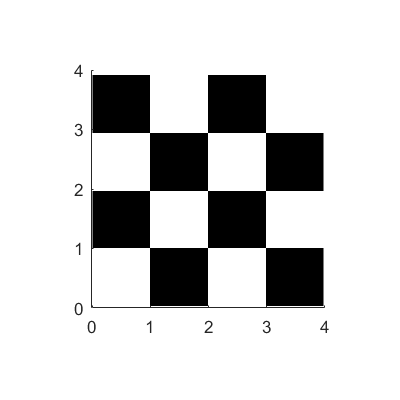
\includegraphics[width = 0.5\textwidth]{images/checkerboard.png}
        \caption{Checkerboard Pattern \label{fig:checkerboard}}
        \label{Q_2dt}
    \end{figure}
    \begin{parts}
    
        \part[2] \textbf{[SOLO]} What is the minimum depth of decision tree that perfectly classifies the $4\times 4$ colored regions in Figure \ref{fig:checkerboard}, using features that only inspect either $x$ or $y$ but not both $x$ and $y$? (How you use each of $x$ and $y$ to construct a feature is up to you.) 

    \begin{your_solution}[title=Your Answer,height=2cm,width=5cm]
    \end{your_solution}
    
    \part[2] \textbf{[SOLO]} What is the minimum depth of decision trees to perfectly classify the colored regions in Figure \ref{fig:checkerboard}, using ANY features of $x$ and $y$? 
    
    \begin{your_solution}[title=Your Answer,height=2cm,width=5cm]
    \end{your_solution}
    
    
    \end{parts}
    
    \clearpage
    Consider the graph below analyzing the size of tree vs. accuracy for a decision tree which has been pruned back to the red line. 
 

\begin{figure}[H]
  \centering
  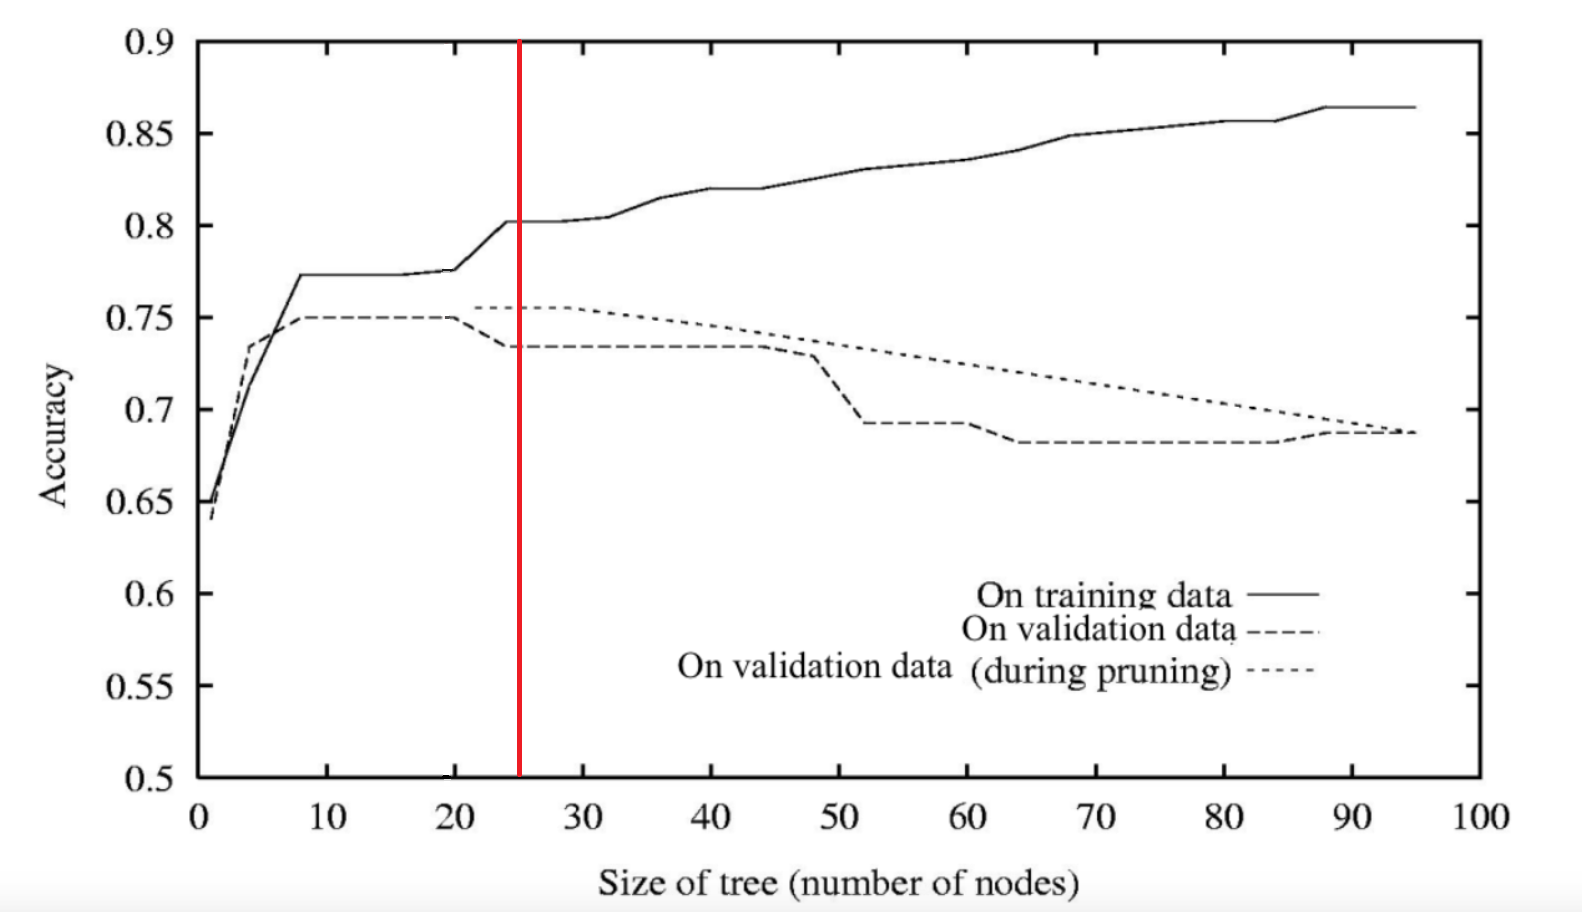
\includegraphics[width = 0.6\textwidth]{images/dtree.png}
  \caption{Pruned decision tree \label{fig:dtree}}
\end{figure}
      

   \question[1] \textbf{[SOLO]} Refer to Figure \ref{fig:dtree}. Let's say that we have a third dataset $D_{new}$ (from the same data distribution), which is not used for training or pruning. 
    
    If we evaluate this new dataset, approximately what is the accuracy when the size of the tree is at 25 nodes, and why? Select one. 
    
    
    \textbf{Select one:}
    \begin{checkboxes}
        \choice Around 0.76 (slightly higher than the accuracy for validation data at 25 nodes)
        \choice Around 0.73 (the same as the accuracy for validation data at 25 nodes)
        \choice Around 0.70 (slightly lower than the accuracy for  validation data at 25 nodes)
        \choice None of the above
    \end{checkboxes}
    
    
    
    
      \question[1] \textbf{[SOLO]} Which of the following gives us the best approximation of the true error? 
   
    
    
 \begin{checkboxes}
        \choice Line corresponding to training data 
        \choice Line corresponding to validation data 
        \choice Line corresponding to new dataset $D_{new}$ 
    \end{checkboxes}
    
    
  
    
    
    
    \question[2] \textbf{[SOLO]} Which of the following are valid ways to avoid overfitting? Select all that apply.

    \textbf{Select all that apply:}
    {
    \checkboxchar{$\Box$} \checkedchar{$\blacksquare$}
    \begin{checkboxes}
        \choice Decrease the training set size. 
        \choice Set a threshold for a minimum number of samples required to split at an internal node. 
        \choice Prune the tree so that cross-validation error is minimal. 
        \choice Maximize the tree depth.
        \choice None of the above.
    \end{checkboxes}
    }

    
    \clearpage
    
    \question[3] \textbf{Ensemble of Decision Tree.} Say we have a dataset shown below. There are 12 data points, with 6 in label "-" and 6 in label "+". We would like to use Decision Trees to solve this binary classification problem. However, in our problem setting, each Decision Tree has access to only ONE line. That is to say, our Decision Tree would have access to only one attribute, and so has max-depth of 1. \\ \\
    By accessing this line, the Decision Tree could know (and only know) whether the data point is on the right side of this line or the left side. (Unofficial definition: let's assume the right side of a line shares the same direction with the \textcolor{OliveGreen}{\textbf{green}} normal vector of that line.) \\ \\
    Finally, please use majority vote strategy to make classification decision at each leaf.\\
    
    \begin{figure}[H]
        \centering
        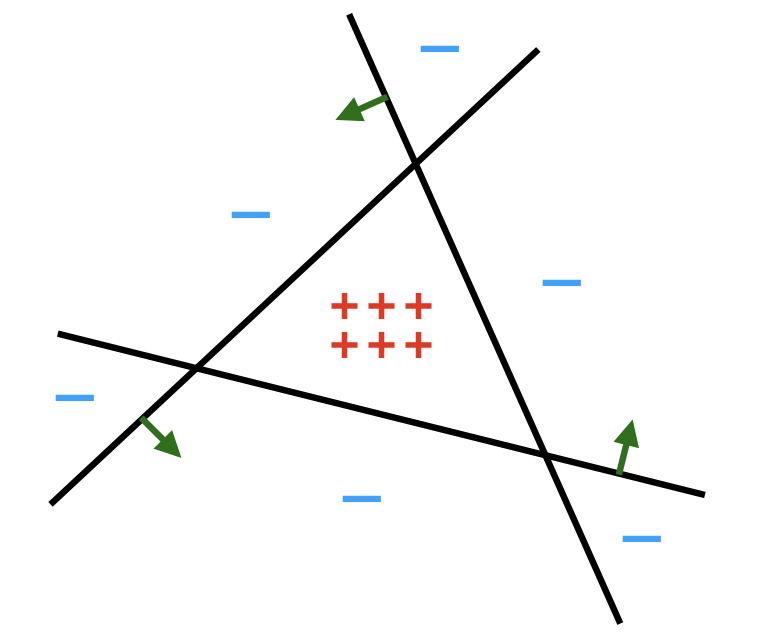
\includegraphics[width = 0.5\textwidth]{images/ensemble_dt.png}
        \label{Q_ensemble_DT}
        \caption{Decision Tree Ensemble \label{fig:ensemble}}
    \end{figure}
    
    \begin{parts}
        \part[1] \textbf{[SOLO]} In Figure \ref{fig:ensemble}, if we train only 1 Decision Tree, what is the best/lowest error rate? Note that we have in total 12 data points. Round to 4 decimal places after the decimal point.
    
    \begin{your_solution}[title=Best/Lowest Error Rate,height=2cm,width=5cm]
    \end{your_solution}
    
        
    \part[2] \textbf{[SOLO]} If we could use 2 Decision Trees in Figure \ref{fig:ensemble}, what is the best/lowest error rate? If we have two Decision Trees, then each would predict each data point with '+' or '-'. Then, we would like to combine these predictions as the final result. If both trees predict '+', then the result is '+'. The same with '-'. However, if one predicts '+' while one predicts '-', then we always choose '-' as the final result to break ties. Round to 4 decimal places after the decimal point.
    
    \begin{your_solution}[title=Best/Lowest Error Rate,height=2cm,width=5cm]
    \end{your_solution}
    
    

\newpage
    \part[2] \textbf{[SOLO]} Now let's train 3 Decision Trees as a forest in Figure \ref{fig:ensemble}. What is the best/lowest error rate? The ensemble strategy is now unanimous voting. That is, if every Decision Tree agrees, then the model predicts a positive label. However, if one of them has a different answer from the other two, then we predict negative. That means, we train each Decision Tree individually, and each Decision Tree choose one unique line as its decision boundary such that it would try its best to achieve maximum accuracy. And, next, if all the Decision Trees agree, then we assign the point a positive label. Round to 4 decimal places after the decimal point.
    
    \begin{your_solution}[title=Best/Lowest Error Rate,height=2cm,width=5cm]
    \end{your_solution}
    
    
    \end{parts}
    
\question[6] Consider a binary classification problem using $1$-nearest neighbors with the Euclidean distance metric. We have $N$ 1-dimensional training points $x^{(1)}, x^{(2)}, \ldots x^{(N)}$ and corresponding labels $y^{(1)}, y^{(2)}, \ldots y^{(N)}$ with $x^{(i)} \in \mathbb{R}$ and $y^{(i)} \in \{0, 1\}$. 
%
Assume the points $x^{(1)}, x^{(2)}, \ldots x^{(N)}$ are in ascending order by value. If there are ties during the 1-NN algorithm, we break ties by choosing the label corresponding to the $x^{(i)}$ with lower value. 
    
    
    \begin{parts} 
    \part[2] \textbf{[GROUP]} Is it possible to build a decision tree that behaves exactly the same as the 1-nearest neighbor classifier? Assume that the decision at each node takes the form of ``$x \leq t$ or $x > t$," where $t \in \mathbb{R}$.
    
    \begin{checkboxes}
        \choice Yes
        \choice No
    \end{checkboxes}
     If your answer is yes, please explain how you will construct the decision tree. If your answer is no, explain why it’s not possible. 
   
    \begin{your_solution}[title=Your answer:,height=6cm,width=15cm]
        
    \end{your_solution}
    
    \clearpage
    \part[2] \textbf{[GROUP]} Let's add a dimension! Now assume the training points are 2-dimensional where $\xv^{(i)} = (x_1^{(i)}, x_2^{(i)}) \in \mathbb{R}^2$ and the decision at each node takes the form of ``$x_j \leq t$ or $x_j > t$," where $t \in \mathbb{R}$ and $j \in \{1,2\}$. Give an example with at most 3 training points for which it isn't possible  to build a decision tree that behaves exactly the same as a 1-nearest neighbor classifier. 

    \begin{your_solution}[title=Your answer:,height=7cm,width=15cm]
    \end{your_solution}
    
    \part [2] \textbf{[GROUP]} Assuming we have 2-dimensional training points $\xv^{(i)} = (x_1^{(i)}, x_2^{(i)}) \in \mathbb{R}^2$ and the decision at each node takes the form of ``$x_j \leq t$ or $x_j > t$," where $t \in \mathbb{R}$ and $j \in \{1,2\}$, under what conditions \textbf{is} it possible to build a decision tree that behaves exactly the same as a 1-nearest neighbor classifier? Explain why it is possible to build the decision tree as stated in part (a) but, in general, not possible in part (b). 

    \begin{your_solution}[title=Your answer:,height=7cm,width=15cm]
    \end{your_solution}
    
    
    \end{parts}
    
\newpage

\end{questions}



\newpage
\section{{\it k}-Nearest Neighbors}


\begin{questions}
    
    \begin{figure}[H]
        \centering
        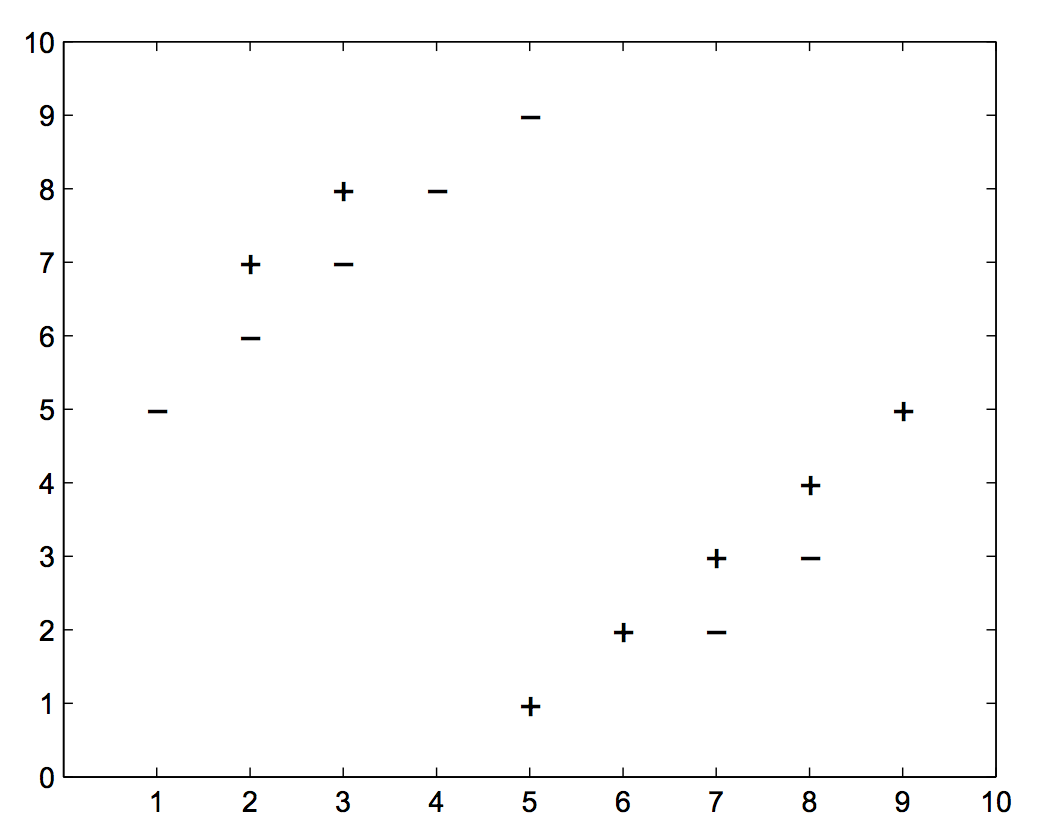
\includegraphics[width = 0.5\textwidth]{images/Q2_knn.png}
        \caption{k-NN Dataset \label{fig:Q2_knn}}
    \end{figure}

    \question[2] \textbf{[SOLO]} Consider a $k$-nearest neighbors ($k$-NN) binary classifier which assigns the class of a test point to be the class of the majority of the $k$-nearest neighbors, according to a Euclidean distance metric. Using Figure \ref{fig:Q2_knn} shown above to train the classifier and choosing $k=6$, what is the classification error on the training set?
    
    Answer as a decimal with precision 4, e.g. (6.051, 0.1230, 1.234e+7)
    
    \begin{your_solution}[title=Your answer:,height=2cm,width=5cm]
    \end{your_solution}
    
    
    %%%%%
    
    

    
    
    \question[1] \textbf{[SOLO]} Again using Figure \ref{fig:Q2_knn}, what is the value of $k$ that minimizes the training error? Let’s assume we break ties by selecting one of the labels uniformly at random.
    
    \begin{your_solution}[title=Your answer:,height=2cm,width=5cm]
    \end{your_solution}

    
    
    \clearpage
    
    \question[2] \textbf{[SOLO]} Let's say that we have a new test point (not present in our training data) $\xv^{\text{new}} = [3,9]^T$ that we would like to apply our $k$-NN classifier to, as seen in figure \ref{fig:Q2_knn_test}.
    
    \begin{figure}[H]
        \centering
        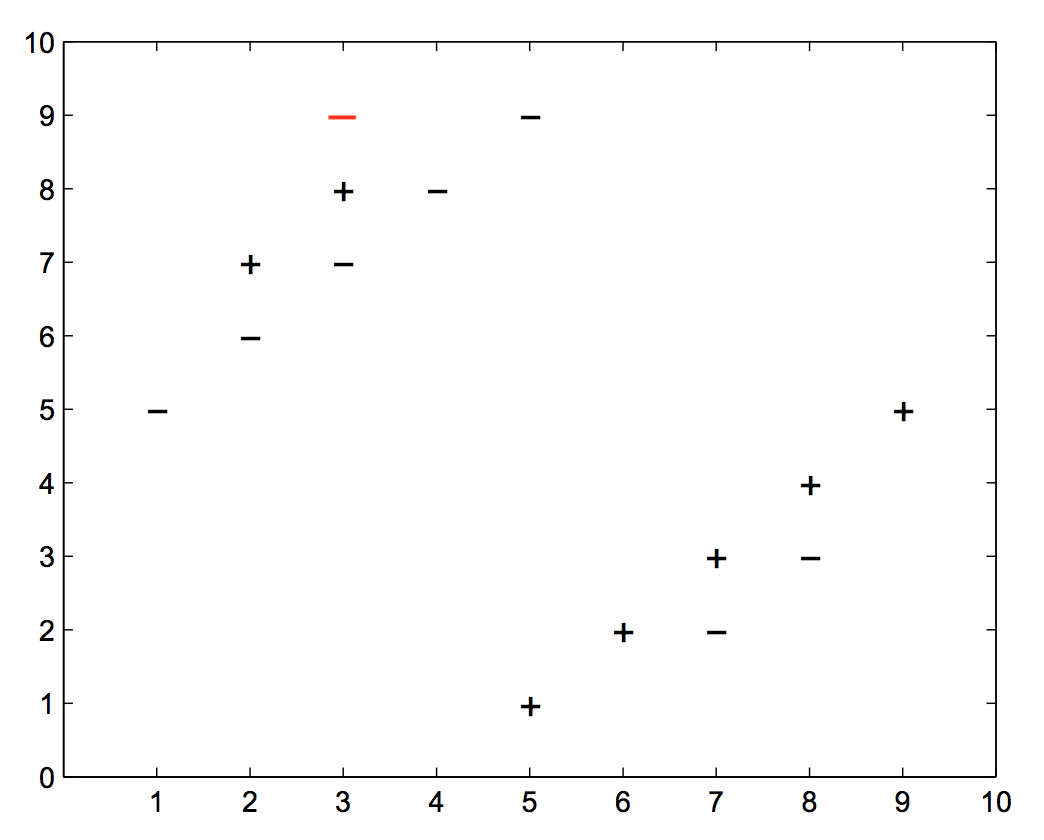
\includegraphics[width = 0.5\textwidth]{images/Q2_knn_test_point.png}
        \caption{k-NN Dataset with Test Point \label{fig:Q2_knn_test}}
    \end{figure}
    
    For which values of $k$ is this test point correctly classified by the $k$-NN algorithm?
    
    \textbf{Select all that apply:}
    {
    \checkboxchar{$\Box$} \checkedchar{$\blacksquare$}
    \begin{checkboxes}
        \choice $k$ = 1
        \choice $k$ = 5
        \choice $k$ = 9
        \choice $k$ = 12
        \choice None of the above
    \end{checkboxes}
    }
    
    
    
    \question[5] Assume we have a training set and a test set drawn from the same distribution, and we would like to classify points in the test set using a $k$-NN classifier. 
    
    \begin{parts}
    
        \part[1] \textbf{[SOLO]} In order to minimize the classification error on this test set, we should always choose the value of $k$ which minimizes the training set error. 
    
    \textbf{Select one:}
    \begin{checkboxes}
        \choice True
        \choice False
    \end{checkboxes}
    
    
    \clearpage
    \part[2] \textbf{[SOLO]} Instead of choosing the hyper-parameters by merely minimizing the training set error, we instead consider splitting the training-all data set into a training and a validation data set, and choose the hyper-parameters that lead to lower validation error. Is choosing hyper-parameters based on validation error better than choosing hyper-parameters based on training error? Justify your opinion with no more than 3 sentences.

    \textbf{Select one:}
    \begin{checkboxes}
        \choice Yes
        \choice No
    \end{checkboxes}
    

     \begin{your_solution}[title=Your answer:,height=5cm,width=15cm]
    \end{your_solution}
    
    \part[2] \textbf{[SOLO]} Your friend Sally suggests that instead of splitting the training set into separate training and validation sets, we should instead use the test set as the validation data for choosing hyper-parameters. Is this a good idea? Justify your opinion with no more than 3 sentences.
    
    \textbf{Select one:}
    \begin{checkboxes}
        \choice Yes
        \choice No
    \end{checkboxes}
    

    \begin{your_solution}[title=Your answer:,height=5cm,width=15cm]
    \end{your_solution}

    \end{parts}
    
    
    \clearpage
    
    \question[3] \textbf{[SOLO]} Consider a binary $k$-NN classifier where $k=4$ and the two labels are ``triangle" and ``square".
    Consider classifying a new point $\xv =(1,1)$, where two of the $\xv$'s nearest neighbors are labeled ``triangle" and two are labeled ``square" as shown below.
    
    \begin{figure}[H]
        \centering
        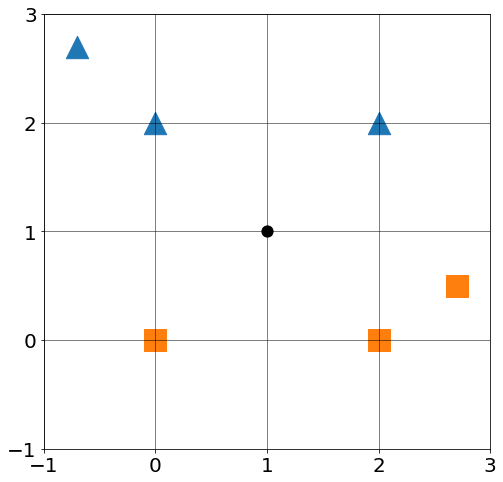
\includegraphics[width = 0.5\textwidth]{images/1-1-5.png}
        \label{Q_5knn}
    \end{figure}
    
    Which of the following methods can be used to break ties or avoid ties on this dataset?
    
    \begin{enumerate}
        \item Assign x the label of its nearest neighbor
        \item Flip a coin to randomly assign a label to $\xv$ (from the labels of its 4 closest points)
        \item Use $k = 3$ instead
        \item Use $k = 5$ instead
    \end{enumerate}

    \textbf{Select one:}
    \begin{checkboxes}
        \choice 1 only
        \choice 2 only
        \choice 2, 3, 4
        \choice 2, 4
        \choice 4 only
        \choice 1, 2, 3, 4
        \choice None of the above
    \end{checkboxes}
    
 
    
    \newpage
    
    \question[2] \textbf{[SOLO]} In this question, we would like to compare the differences among $k$-NN, the perceptron algorithm, and linear regression.
    
    {
    \checkboxchar{$\Box$} \checkedchar{$\blacksquare$}
    \textbf{Select all that apply:}
    \begin{checkboxes}
        \choice For classification tasks, both $k$-NN and the perceptron algorithm can have linear decision boundaries.
        \choice For classification tasks, both $k$-NN and the perceptron algorithm always have linear decision boundaries.
        \choice All three models can be susceptible to overfitting.
        \choice In all three models, after the training is completed, we must store the training data to make predictions on the test data.
        \choice None of the above.
    \end{checkboxes}
    }

    

    \question[3] \textbf{[SOLO]} Please select all that apply about $k$-NN in the following options. \\ \textbf{Select all that apply:}
    {
    \checkboxchar{$\Box$} \checkedchar{$\blacksquare$}
    \begin{checkboxes}
        \choice A larger $k$ gives a smoother decision boundary.
        \choice To reduce the impact of noise or outliers in our data, we should increase the value $k$.
        \choice If we make $k$ too large, we could end up overfitting the data.
        \choice We can use cross-validation to help us select the value of $k$.
        \choice We should never select the $k$ that minimizes the error on the validation dataset.
        \choice None of the above.
    \end{checkboxes}
    }

    
    
    \newpage
    
    \question[8] Consider the following data concerning the relationship between academic performance and salary after graduation. High school GPA and university GPA are two numerical predictors and salary is the numerical target. Note that salary is measured in thousands of dollars per year.
    
    \begin{table}[H]
        \centering
        \begin{tabular}{cccc}
            \textbf{Student ID} & \textbf{High School GPA} & \textbf{University GPA} & \textbf{Salary} \\
            1 & 2.5 & 3.8 & 45 \\
            2 & 3.6 & 2.4 & 55 \\
            3 & 3.3 & 3.5 & 91 \\
            4 & 4.0 & 4.0 & 142 \\
            5 & 2.2 & 3.2 & 88 \\
            6 & 3.8 & 3.0 & 2600 \\
            7 & 3.0 & 2.0 & 163 \\
            8 & 3.3 & 2.8 & 67 \\
            9 & 3.9 & 3.8 & unknown \\
        \end{tabular}
        \label{tab:my_label}
    \end{table}
    
    \begin{parts}
    \part[2] \textbf{[GROUP]} Among Students 1 to 8, who is the nearest neighbor to Student 9, using Euclidean distance? Answer the Student ID only.
    
    \begin{your_solution}[title=Your answer:,height=2cm,width=5cm]
    \end{your_solution}
    
    
    
    \part[3] \textbf{[GROUP]} Now, our task is to predict the salary Student 9 earns after graduation. We apply $k$-NN to this regression problem: the prediction for the numerical target (salary in this example) is equal to the average of salaries for the top $k$ nearest neighbors. If $k=4$, what is our prediction for Student 9's salary? Round your answer to the nearest integer. Be sure to use the same unit of measure (thousands of dollars per year) as the table above.
    
    \begin{your_solution}[title=Your answer:,height=2cm,width=5cm]
    \end{your_solution}
    
    

    \part[2] \textbf{[GROUP]} Suppose that the first 8 students shown above are only a subset of your full training data set, which consists of 10,000 students. We apply $k$-NN regression using Euclidean distance to this problem and we define training loss on this full data set to be the mean squared error (MSE) of salary. Now consider the possible consequences of modifying the data in various ways. Which of the following changes \textbf{could} have an effect on training loss on the full data set as measured by mean squared error (MSE) of salary?
    
    
        
    \textbf{Select all that apply:}
    {
    \checkboxchar{$\Box$} \checkedchar{$\blacksquare$}
    \begin{checkboxes}
        \choice Rescaling only ``High School GPA" to be a percentage of 4.0
        \choice Rescaling only ``University GPA" to be a percentage of 4.0
        \choice Rescaling both ``High School GPA" and ``University GPA", so that each is a percentage of 4.0
        \choice None of the above.
    \end{checkboxes}
    }

    
    
    \end{parts}
   
    \clearpage
    
    \question[3] \textbf{[GROUP]} Suppose we have $N$ training examples, and each one has $M$ features. Derive the prediction time complexity of running a naive $k$-NN binary classifier with Euclidean distance on one test point (for a fixed $k$) and use pseudo-code to justify your explanation.
    
    \begin{your_solution}[title=Your answer:,height=10cm,width=15cm]
    \end{your_solution}
    
    
    \question[3] \textbf{[GROUP]} We have been dealing with k-NN with features that are all continuous values. Can we use k-NN on a data set that has categorical features that take three or more values? If yes, what is a distance metric that could be used to compute distance between categorical data points. Explain your reasoning.
    
    \begin{your_solution}[title=Your answer:,height=5cm,width=15cm]
    \end{your_solution}
    
    \clearpage
\end{questions}
\section{Perceptron}
\begin{questions}
    \question[1] \textbf{[SOLO]} Consider running the online perceptron algorithm on some sequence of examples $S$ (an example is a data point and its label). Let $S^\prime$ be the same set of examples as $S$, but presented in a different order.
    
    True or False: the online perceptron algorithm is guaranteed to make the same number of mistakes on $S$ as it does on $S^\prime$.

    \textbf{Select one:}
    \begin{checkboxes}
        \choice True
        \choice False
    \end{checkboxes}


    
    \question[3] \textbf{[SOLO]} Suppose we have a perceptron whose inputs are 2-dimensional vectors and each feature vector component is either 0 or 1, i.e., $x_i \in \{0,1\}$. The prediction function $y = \operatorname{sign}(w_1x_1 + w_2x_2 + b)$, and
    $$
    \operatorname{sign}(z) = 
    \begin{cases}
    1, & \textrm{ if } z \geq 0\\
    0, & \textrm{ otherwise}.
    \end{cases}
    $$
    Which of the following functions can be implemented with the above perceptron? That is, for which of the following functions does there exist a set of parameters $w,b$ that correctly define the function. 
    \textbf{Select all that apply:}
    {
    \checkboxchar{$\Box$} \checkedchar{$\blacksquare$}
    \begin{checkboxes}
        \choice AND function, i.e., the function that evaluates to 1 if and only if all inputs are 1, and 0 otherwise.
        \choice OR function, i.e., the function that evaluates to 1 if and only if at least one of the inputs are 1, and 0 otherwise.
        \choice XOR function, i.e., the function that evaluates to 1 if and only if the inputs are not all the same. For example
        $$
        \operatorname{XOR}(1,0) = 1, \textrm{ but } \operatorname{XOR}(1,1) = 0.
        $$
        \choice None of the above.
    \end{checkboxes}
    }

    
    
    
    \question[2] \textbf{[SOLO]} Suppose we have a dataset $\left\{ \left(\xv^{(1)},y^{(1)}\right),\ldots, \left(\xv^{(N)},y^{(N)}\right) \right\}$, where $\xv^{(i)} \in \mathbb{R}^M$, $y^{(i)}\in\{+1,-1\}$. We would like to apply the perceptron algorithm on this dataset. Assume there is no intercept term. How many parameter values is the perceptron algorithm learning?

    \textbf{Select one:}
    \begin{checkboxes}
        \choice $N$
        \choice $N\times M$
        \choice $M$
    \end{checkboxes}


    
    \clearpage
    
    \question[2] \textbf{[SOLO]} Which of the following are true about the perceptron algorithm?

    \textbf{Select all that apply:}
    {%
    \checkboxchar{$\Box$} \checkedchar{$\blacksquare$}
    \begin{checkboxes}
        \choice The number of mistakes the perceptron algorithm makes is proportional to the number of points in the dataset. 
        \choice The perceptron algorithm converges on any dataset.
        \choice The perceptron algorithm can be used in the context of online learning.
        \choice For linearly separable data, the perceptron algorithm always finds the separating hyperplane with the largest margin.
        \choice None of the above.
    \end{checkboxes}
    }

    
    
    
    \question[2] \textbf{[SOLO]} The following table shows a data set and the number of times each point is misclassified during a run of the perceptron algorithm. What is the separating plane $w$ found by the algorithm, i.e. $w = [b, w_1, w_2, w_3]$? Assume that the initial weights are all zero.
  
  \begin{table}[H]
    \centering
        \begin{tabular}{|l|l|l|l|l|}
         $x_1$ & $x_2$ & $x_3$ & $y$ & \text{Times Misclassified} \\ \hline
        2 & 1 & 5 & 1 & 10 \\ \hline
        5 & 3 & 3 & 1 & 5 \\ \hline 
        4 & 1 & 2 & 1 & 8 \\ \hline 
        8 & 4 & 8 & -1 & 2 \\ \hline 
        3 & 2 & 6 & -1 & 3 \\ \hline 
        \end{tabular}
    \end{table}
    
    \textbf{Select one:}
    \begin{checkboxes}
        \choice $[3,22,11,24]$ 
        \choice $[0,-5,20,-10]$ 
        \choice $[16,56,18,47]$ 
        \choice $[18,52,19,47]$ 
    \end{checkboxes}
    
    
    
    

    
    \question[2] \textbf{[SOLO]} Please select the correct statement(s) about the mistake bound of the perceptron algorithm. 

    \textbf{Select all that apply:}
    {%
    \checkboxchar{$\Box$} \checkedchar{$\blacksquare$}
    \begin{checkboxes}
        \choice If the minimum distance from any data point to the separating hyperplane is increased, without any other change to the data points, the mistake bound will also increase.
        \choice If the whole dataset is shifted away from origin, then the mistake bound will also increase.
        \choice If the size of the data set (i.e., the maximum pair-wise distance between data points) is increased, then the mistake bound will also increase.
        \choice The mistake bound is linearly inverse-proportional to the minimum distance of any data point to the separating hyperplane of the data.
        \choice None of the above.
    \end{checkboxes}
    }



    \clearpage

    \question[2] \textbf{[SOLO]} Suppose we have data whose elements are of the form $[x_1,x_2]$, where $x_1 - x_2 = 0$. We do not know the label for each element. Suppose the perceptron algorithm starts with $\bm{\theta} = [3,5]$, which of the following values will $\bm{\theta}$ never take on in the process of running the perceptron algorithm on the data?

    \textbf{Select one:}
    \begin{checkboxes}
        \choice $[-1,1]$
        \choice $[4,6]$
        \choice $[-3,0]$
        \choice $[-6,-4]$
    \end{checkboxes}

    
    \question[2] \textbf{[SOLO]} Consider the linear decision boundary below and the training dataset shown. Which of the following are valid weights $\bm{\theta}$ and its corresponding training error? (Note: Assume the decision boundary is fixed and does not change while evaluating training error.)
    
    \textbf{Select all that apply:}
    {%
    \checkboxchar{$\Box$} \checkedchar{$\blacksquare$}
    \begin{checkboxes}
        \choice $\bm{\theta} = [2,1]$, error  = 5/13
        \choice $\bm{\theta} = [-2,1]$, error = 5/13
        \choice $\bm{\theta} = [2,-1]$, error = 8/13
        \choice $\bm{\theta} = [2,-1]$, error = 5/13
        \choice $\bm{\theta} = [-2,1]$, error = 8/13
        \choice $\bm{\theta} = [-2,-1]$, error = 8/13
        \choice None of the above.
    \end{checkboxes}
    }
    
    
    \begin{figure}[H]
        \centering
        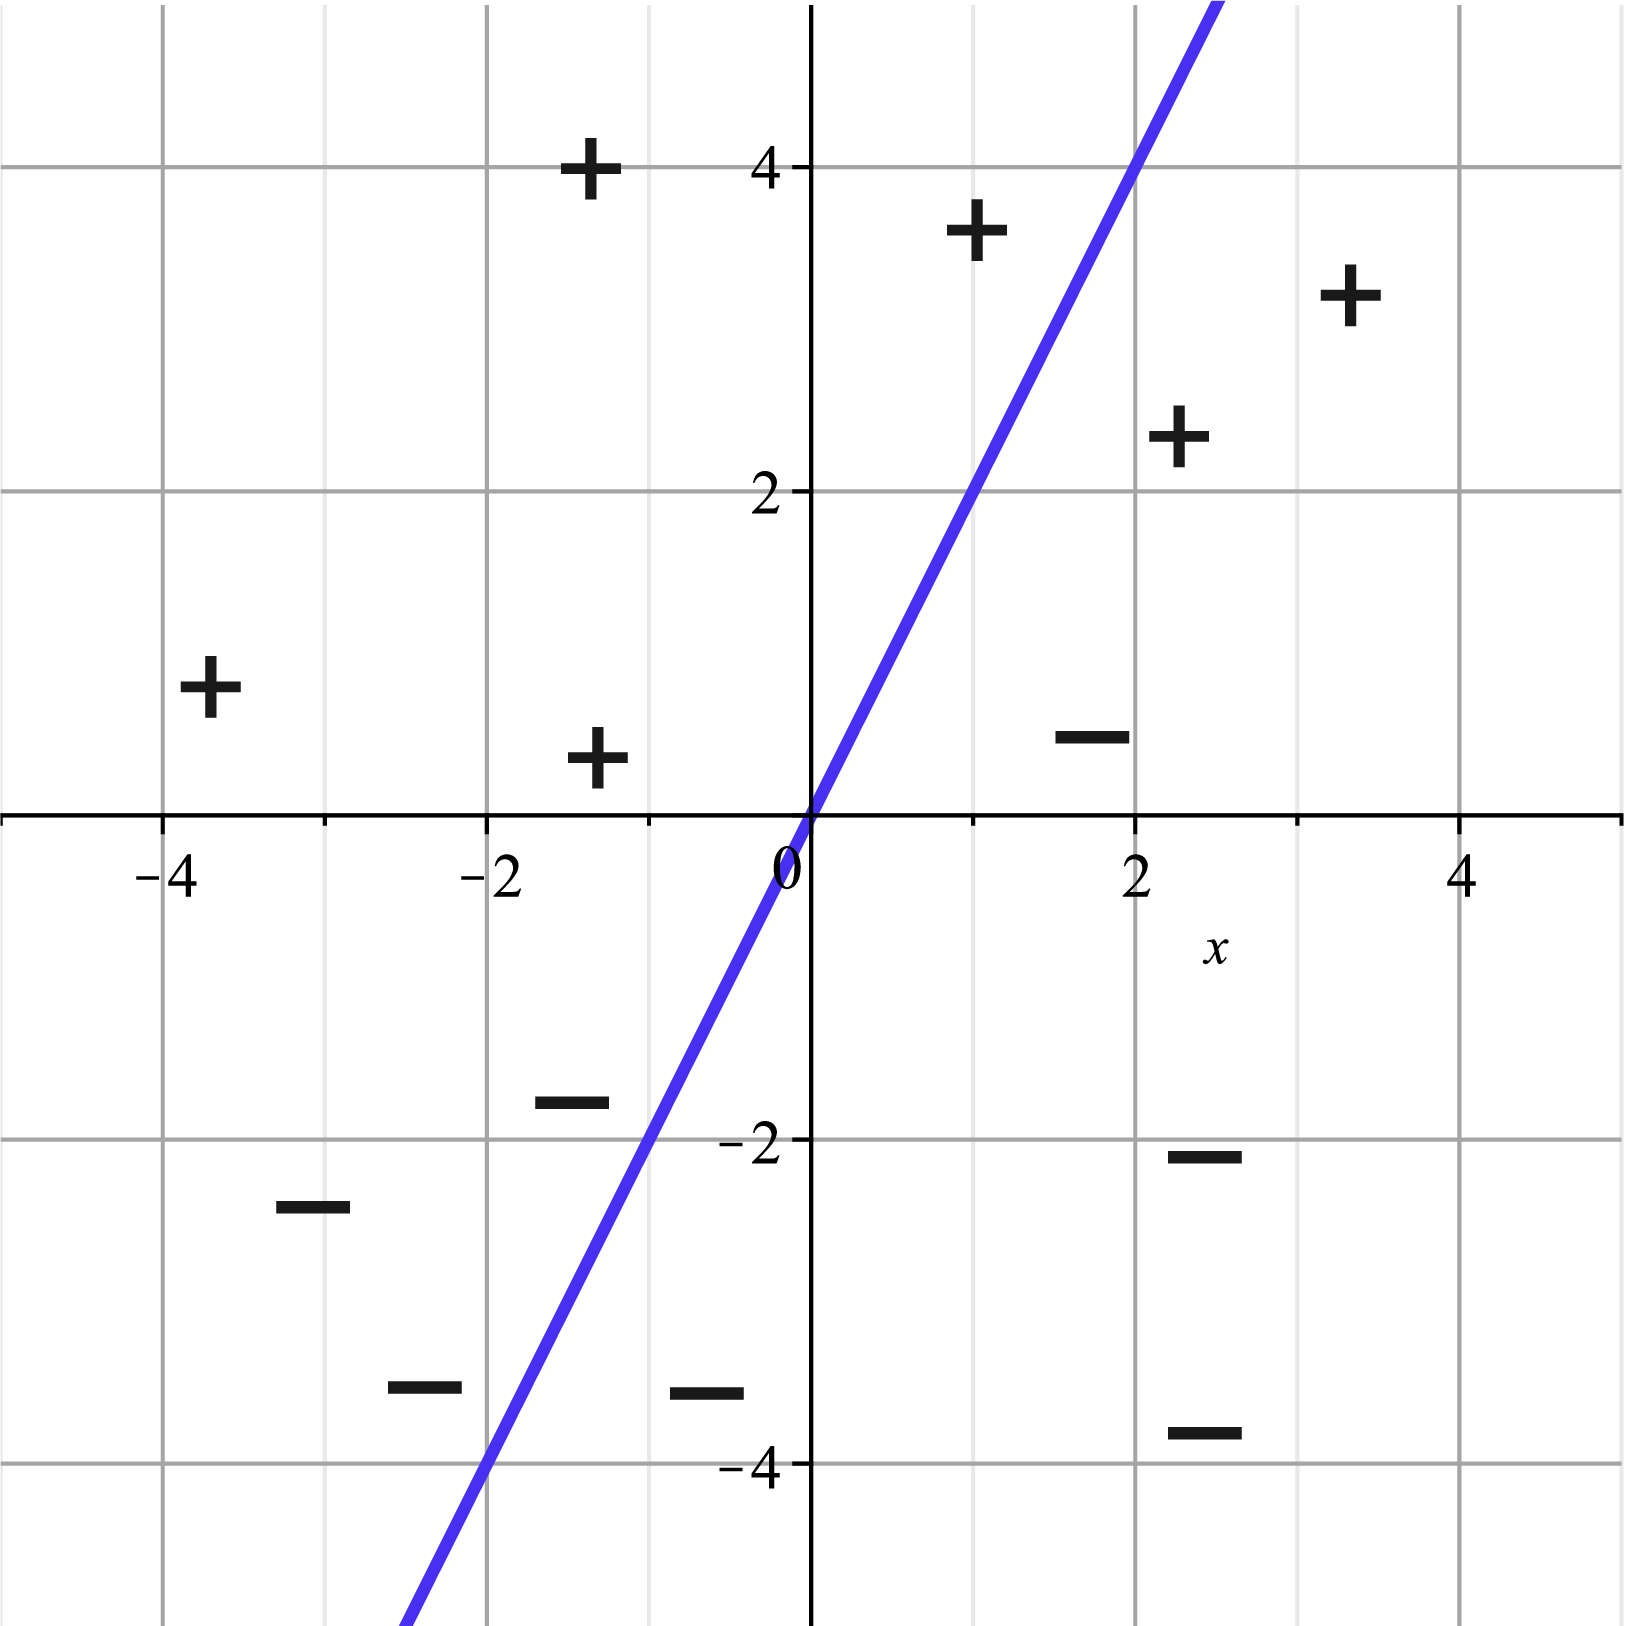
\includegraphics[width = 0.5\textwidth]{images/perceptron_boundary.png}
        \label{Q_10perceptron}
    \end{figure}
    
    
    \clearpage
    
    
    \question[9] The following problem will walk you through an application of the Perceptron Mistake Bound. The following table shows a linearly separable dataset. Your task will be to determine the mistake bound for the dataset below. Then, you will run the training of the perceptron.
    
    \begin{center}
    \begin{tabular}{||c c c||}
        \hline
         $x_1$ & $x_2$ & $y$ \\ [0.5ex]
        \hline\hline
        -1.939 & 2.704 & 1 \\
        \hline
        -0.928 & -3.054 & -1 \\
        \hline
        -2.181 & -3.353 & -1 \\
        \hline
        -0.142 & 1.440 & 1 \\
        \hline
        2.605 & -0.651 & 1 \\
        \hline
    \end{tabular}
    \end{center}
    
    \begin{parts}
        \part[2] \textbf{[SOLO]} Compute the radius R of the "circle" which bounds the data points. Round your answer to 3 decimal places after the decimal point. 
        
        \begin{your_solution}[title=Radius:,height=2cm,width=5cm]
        \end{your_solution}
        
        
        
        \part[2] \textbf{[SOLO]} Assume that the linear separator with the largest margin is given by \[\thetav^{*T}\begin{bmatrix}
        x \\
        y \\ 
        1
        \end{bmatrix} = 0, \text{, where } \thetav^* = \begin{bmatrix}
        3 \\
        4 \\ 
        5
        \end{bmatrix}
        \]
        Now, compute the margin of the dataset. Round your answer to 3 decimal places after the decimal point. 
        
        \begin{your_solution}[title=Margin:,height=2cm,width=5cm]
        \end{your_solution}
        
        
        
        \part[1] \textbf{[SOLO]} Based on the above values, what is the theoretical perceptron mistake bound for this dataset, given this linear separator? Round your answer to 3 decimal places after the decimal point.
        
        \begin{your_solution}[title=Mistake Bound:,height=2cm,width=5cm]
        \end{your_solution}
        
        
        
        \clearpage
        
        \part[3] \textbf{[SOLO]} Finally, train the perceptron using the dataset. Train using the datapoints \textbf{in the given order, top to bottom} repeatedly until convergence. Give the final weights in a comma-separated list ( $w_1$, $w_2$, $b$ ).
        
        \begin{your_solution}[title=Weights:,height=2cm,width=5cm]
        \end{your_solution}
        
        
        
        \part[1] \textbf{[SOLO]} How many mistakes did the perceptron make? 
        
        \begin{your_solution}[title=Mistakes:,height=2cm,width=5cm]
        \end{your_solution}
        
        
        
    \end{parts}
    \clearpage
\end{questions}
\section{Linear Regression}
\begin{questions}

    \question[3] We would like to fit a linear regression estimate to the dataset 
    $$
    D = \left\{\left(\xv^{(1)},y^{(1)}\right), \left(\xv^{(2)},y^{(2)}\right),\cdots, \left(\xv^{(N)},y^{(N)}\right)\right\}
    $$ with $\xv^{(i)} \in \mathbb{R}^M$ by minimizing the ordinary least square (OLS) objective function:
    $$
    J(\wv) = \frac{1}{2}\sum_{i=1}^N\left(y^{(i)} - \sum_{j=1}^M w_j x_j^{(i)}\right)^2
    $$

    \begin{parts}
        \part[2] \textbf{[SOLO]} Specifically, we solve for each coefficient $w_k$ ($1\leq k\leq M$) by deriving an expression of $w_k$ from the critical point $\frac{\partial J(\wv)}{\partial w_k} = 0$. What is the expression for each $w_k$ in terms of the dataset 
    $(\xv^{(1)},y^{(1)}), \cdots, (\xv^{(N)},y^{(N)})$ and $w_1,\cdots,w_{k-1},w_{k+1},\cdots,w_M$?
    
    \textbf{Select one:}
    \begin{checkboxes}
        \choice $w_k = \frac{\sum_{i=1}^N x_k^{(i)}(y^{(i)}-\sum_{j=1,j\neq k}^M w_j x_j^{(i)})}{\sum_{i=1}^N (x_k^{(i)})^2}$
        \choice $w_k = \frac{\sum_{i=1}^N x_k^{(i)}(y^{(i)}-\sum_{j=1,j\neq k}^M w_j x_j^{(i)})}{\sum_{i=1}^N (y^{(i)})^2}$
        \choice $w_k = \sum_{i=1}^N x_k^{(i)}(y^{(i)}-\sum_{j=1}^M w_j x_j^{(i)})$
        \choice $w_k = \frac{\sum_{i=1}^N x_k^{(i)}(y^{(i)}-\sum_{j=1,j\neq k}^M w_j x_j^{(i)})}{\sum_{i=1}^N (x_k^{(i)} y^{(i)})^2}$
    \end{checkboxes}

    
    
    \part[1] \textbf{[SOLO]} How many coefficients do you need to estimate? When solving for these coefficients, how many equations do you have?
    
    \textbf{Select one:}
    \begin{checkboxes}
        \choice $N$ coefficients, $M$ equations
        \choice $M$ coefficients, $N$ equations
        \choice $M$ coefficients, $M$ equations
        \choice $N$ coefficients, $N$ equations
    \end{checkboxes}
    
    \end{parts}
    
    \clearpage
    
    \question[3] \textbf{[SOLO]} Consider the following 3 data points for linear regression: $\xv^{(1)} = [0, 1, 2]^T$, $\xv^{(2)} = [1, 0, 2]^T$ and $\xv^{(3)} = [2, 1, 0]^T$. The corresponding y values are $y^{(1)}=3$, $y^{(2)}=6$, $y^{(3)}=9$.
    
    Assume the intercept to be 0. Find the weights $\thetav = [\theta_1,  \theta_2,  \theta_3]^T \in \mathbb{R}^3$ such that the mean squared error $J(\thetav) = (\mathbf{\yv} - \Xv \thetav)^T(\mathbf{\yv} - \Xv \thetav)$ is minimized on this training set. $\Xv$ is the design matrix where $\Xv_{ij} = \xv_j^{(i)}$. 
    
    \begin{your_solution}[title=$\theta_1$:,height=2cm,width=5cm]
    \end{your_solution}
    \begin{your_solution}[title=$\theta_2$:,height=2cm,width=5cm]
    \end{your_solution}
    \begin{your_solution}[title=$\theta_3$:,height=2cm,width=5cm]
    \end{your_solution}
    
    
    

    \question[1] \textbf{[SOLO]} Assume that a data set has $M$ data points and $N$ variables, where $M>N$. Different loss functions would return the same sets of solutions as long as they are convex.
    
    \textbf{Select one:}
    \begin{checkboxes}
        \choice True
        \choice False
    \end{checkboxes}
    
    
    
\question[1] \textbf{[SOLO]} Suppose we are working with datasets where the number of features is 3. The optimal solution for linear regression is always unique regardless of the number of data points that are in this dataset.
    
    \textbf{Select one:}
    \begin{checkboxes}
        \choice True
        \choice False
    \end{checkboxes}
    
    
    \question[1] \textbf{[SOLO]} Consider the following dataset:
        \begin{table}[H]
    \centering
        \begin{tabular}{llllll}
        $x_1$ & 1.5 & 2.5 & 3.5 & 4.5 & 5.5 \\
        $x_2$ & 3.0 & 5.0 & 7.0 & 9.0 & 11.0 \\
        y & 4.0 & 7.0 & 8.0 & 11.0 & 17.0
        \end{tabular}
    \end{table}
   We want to carry out a multiple-linear regression between $y$ (dependent variable) and $x_1$ and $x_2$ (independent variables). The closed-form solution given by $\wv = \left(\Xv^T\Xv\right)^{-1}\Xv^T \Yv$ will return the unique solution. 
    \\~\\
    Note: The $i^{\text{th}}$ row of $\Xv$ contains the $i^{\text{th}}$ data point $(x_1^{(i)}, x_2^{(i)})$ while the $i^{\text{th}}$ row of $\Yv$ contains the $i^{\text{th}}$ data point $y^{(i)}$. 
    
        \textbf{Select one:}
    \begin{checkboxes}
        \choice True
        \choice False
    \end{checkboxes}
    
    
    \clearpage
    
     \question[3] \textbf{[SOLO]} Identifying whether a function is a convex function is useful because a convex function's local minimum has the nice property that it has to be the global minimum. Please select all functions below that are convex functions. Note $dom(f)$ denotes the domain of the function $f$. \\
        {%
    \checkboxchar{$\Box$} \checkedchar{$\blacksquare$}
    \textbf{Select all that apply:}
    \begin{checkboxes}
        \choice $f(x) = x^3 + 3x + 7, dom(f) = \mathbb{R}$
        \choice $f(x) = -\log x, dom(f) = \mathbb{R}_{++}$ (the set of positive real numbers)
        \choice $f(x) = -|x|, dom(f) = \mathbb{R}$
        \choice $f(x) = -2x^2, dom(f) = \mathbb{R}$
        \choice $f(x) = ||\xv||_2^2,\, dom(f) = \mathbb{R}^n$
        \choice None of the above.
    \end{checkboxes}
    }


    \question[2] \textbf{[GROUP]} Typically we can solve linear regression problems in two ways. One is through direct methods, e.g. solving the closed form solution, and the other is through iterative methods (gradient descent). Consider a linear regression on data $(\Xv, \yv)$. We assume each row in $\Xv$ denotes one input in the dataset. Please select all correct options.
    
    \textbf{Select all that apply:}
        {%
    \checkboxchar{$\Box$} \checkedchar{$\blacksquare$}
    \begin{checkboxes}
        \choice If the matrix $\Xv^T\Xv$ is invertible, the exact solution is always preferred for solving the solution to linear regression as computing matrix inversions and multiplications are fast regardless of the size of the dataset.
        \choice Assume $N$ is the number of examples and $M$ is the number of features. The computational complexity of $N$ iterations of batch gradient descent is $O(MN)$.
        \choice The computational complexity of the closed form solution is linear in number of parameters/features.
        \choice None of the above.
    \end{checkboxes}
    }
    
    
    
    \newpage
    
    \question[8] \label{Q7_linear_regression} Consider the following dataset:
    \begin{table}[H]
    \centering
        \begin{tabular}{llllll}
        x & 9.0 & 2.0 & 6.0 & 1.0 & 8.0 \\
        y & 1.0 & 0.0 & 3.0 & 0.0 & 1.0
        \end{tabular}
    \end{table}
    Let $x$ be the vector of datapoints and $y$ be the label vector. Here, we are fitting the data using gradient descent. Note that our objective function is $\frac{1}{N}\sum_{i=1}^N (wx_i + b - y_i)^2$ where $N$ is the number of data points, $w$ is the weight, and $b$ is the intercept.
    
    \begin{parts}
        \part[2] \textbf{[GROUP]} If we initialize the weight as $3.0$ and intercept as $0.0$, what is the gradient of the loss function with respect to the weight $w$, calculated over all the data points, in the first step of the gradient descent update? Round to 2 decimal places after the decimal point.
        
        \begin{your_solution}[title=Gradient:,height=2cm,width=6cm]
    \end{your_solution}
    
    
    \part[4] \textbf{[GROUP]} Compute the direct solution of the weight and the intercept for the objective function defined in the previous question. Round to 2 decimal places after the decimal point.
    
    \begin{your_solution}[title=Weight:,height=2cm,width=6cm]
    \end{your_solution}
    
    
    \part[2] \textbf{[GROUP]} Let the learning rate be $0.001$. Perform five steps of batch gradient descent on the data. Fill in the blank with the value of the weight after five steps of batch gradient descent. Round to 2 decimal places after the decimal point.
    
    \begin{your_solution}[title=Weight:,height=2cm,width=6cm]
    \end{your_solution}
    
    
    
    
    \end{parts}

    \clearpage
    
    \question[6] Consider a dataset $D = \big((x^{(1)}, y^{(1)}), \ldots, (x^{(n)}, y^{(n)}) \big)$ and the solution to linear regression on $D$ is $y = w_1 x + b_1$. 
    
    \begin{parts}
        \part[2] \textbf{[GROUP]} Now, suppose we have the dataset
        ${(x^{(1)} + \alpha, y^{(1)} + \beta), \ldots, (x^{(n)} + \alpha, y^{(n)} + \beta)}$ where $\alpha > 0, \beta > 0$ and $w_1 \alpha \neq \beta$. The solution to the linear regression on this dataset is $y = w_2 x + b_2$. Select the correct statement about $w_1, w_2, b_1, b_2$ below. Note that the statement should hold no matter what values $\alpha, \beta$ take on within the specified constraints.
    
        \textbf{Select one:}
        \begin{checkboxes}
            \choice $w_1 = w_2, b_1 = b_2$
            \choice $w_1 \neq w_2, b_1 = b_2$
            \choice $w_1 = w_2, b_1 \neq b_2$
            \choice $w_1 \neq w_2, b_1 \neq b_2$
        \end{checkboxes}
        
    
        
        \part[2] \textbf{[GROUP]} Let $\Bar{x}$ and $\Bar{y}$ be the mean of the x and y coordinates, respectively. After mean centering the dataset to create $D_{new} =\big((x^{(1)} - \Bar{x}, y^{(1)} - \Bar{y}), \ldots, (x^{(n)} - \Bar{x}, y^{(n)} - \Bar{y}) \big)$, let the solution to linear regression on $D_{new}$ be $y = w_3 x + b_3$. Explain how $w_3$ compares to $w_1$ and justify.
        
        \begin{your_solution}[title=Your answer:,height=4cm,width=15cm]
        \end{your_solution}
        
        
        \part[2] \textbf{[GROUP]} We decide to ask a friend to analyze $D$; however, he makes a mistake by duplicating a subset of the rows in $D$.  Explain why his solution to linear regression on the duplicated data may differ from the solution to linear regression on $D$.
        
        \begin{your_solution}[title=Your answer:,height=4cm,width=15cm]
        \end{your_solution}
        
        
    \end{parts}
    
\end{questions}



\clearpage
    
\section{Collaboration Questions}
After you have completed all other components of this assignment, report your answers to these questions regarding the collaboration policy. Details of the policy can be found \href{http://www.cs.cmu.edu/~mgormley/courses/10601/syllabus.html}{here}.
\begin{enumerate}
    \item Did you receive any help whatsoever from anyone in solving this assignment? If so, include full details.
    \item Did you give any help whatsoever to anyone in solving this assignment? If so, include full details.
    \item Did you find or come across code that implements any part of this assignment ? If so, include full details.
\end{enumerate}

\begin{your_solution}[height=6cm]
% YOUR ANSWER 

\end{your_solution}    

\end{document}